% document style header
\documentclass[a4paper, 12pt]{config/homework}

% import default packages
\usepackage{config/defpackages}
% import custom math commands
\usepackage{config/domath}

% end preamble
\begin{document}

% document title
\noindent
\begin{tabularx}{\textwidth}{>{\centering\arraybackslash}X>{\centering\arraybackslash}X>{\centering\arraybackslash}X}
Calvin Sprouse & PHYS474 Homework 6 & 2024 February 22\\
\midrule
\end{tabularx}

% homework problems begin
\begin{enumerate}
\item Consider a particle interacting with the potential barrier:
\[V(x) = \begin{cases}
0, & x < 0, \\ V_0, & x > 0.
\end{cases}\]
What kinds of wavefunction solutions are possible?
% I am looking for a qualitative discussion rather than calculations

Free particle wavefunctions are possible solutions to this potential.
In the region \(x<0\) we have the typical free particle condition \(V(x)=0\).
At the barrier there exist reflected and transmitted components of the free particle solution.
In the region \(x>0\) free particle solutions can exist only if the particle energy is greater than the potential.
There will be no bound state solutions only scattering state solutions.

\vspace{\baselineskip}
\item We calculated the even bound-state wavefunctions for the finite-square well in class. Now, preform this calculation for the odd wavefunction solutions. By determining the wavefunction and apply appropriate boundary conditions, calculate the transcendental equation that will allow you to determine the bound-state energies. Use \(Z = \ell a\), and \(Z_0 = \frac{a}{\hbar}\sqrt{2mV_0}\) to express your transcendental equation more compactly.
Plot the left- and right-hand sides of the equation as a function of \(Z\) for \(Z_0=2\). How many bound sates with odd wavefunctions are there for \(Z_0=2\)?

We can begin with Griffiths Equation 2.154 where we have chosen the odd solutions by replacing the \(\cos\) term with the corresponding \(\sin\) term. Then,
\[\psi(x) = \begin{cases}
F\exp(-\kappa x), & x > a, \\ C\sin(lx), & 0 < x < a, \\ \psi(-x), & x < 0.
\end{cases}\]
The boundary condition of continuity of \(\psi\) at \(x=a\) requires that
\[F\exp(-\kappa a) = C\sin(la),\]
and continuity of \(\diff{\psi}{x}\) requires that
\[-\kappa F \exp(-\kappa a) = l C \cos(la).\]
Dividing the boundary condition requirement of the derivative by the boundary condition requirement of \(\psi\) yields
\[\kappa = -l\cot(la).\]
From Griffiths Equations 2.149 and 2.151
\[\kappa a = \sqrt{z_0^2 - z^2}.\]
Then,
\[\kappa a = - la \cot(la)\]
becomes
\[\sqrt{\frac{z_0^2}{z^2} - 1} = -\cot(z).\]
We take \(Z_0=2\) and find the number of bound states with odd wavefunctions at this particular \(Z_0\). Thus,
\[-\cot(z) = \sqrt{\frac{4}{z^2}-1}.\]
\begin{figure}[H]
    \centering
    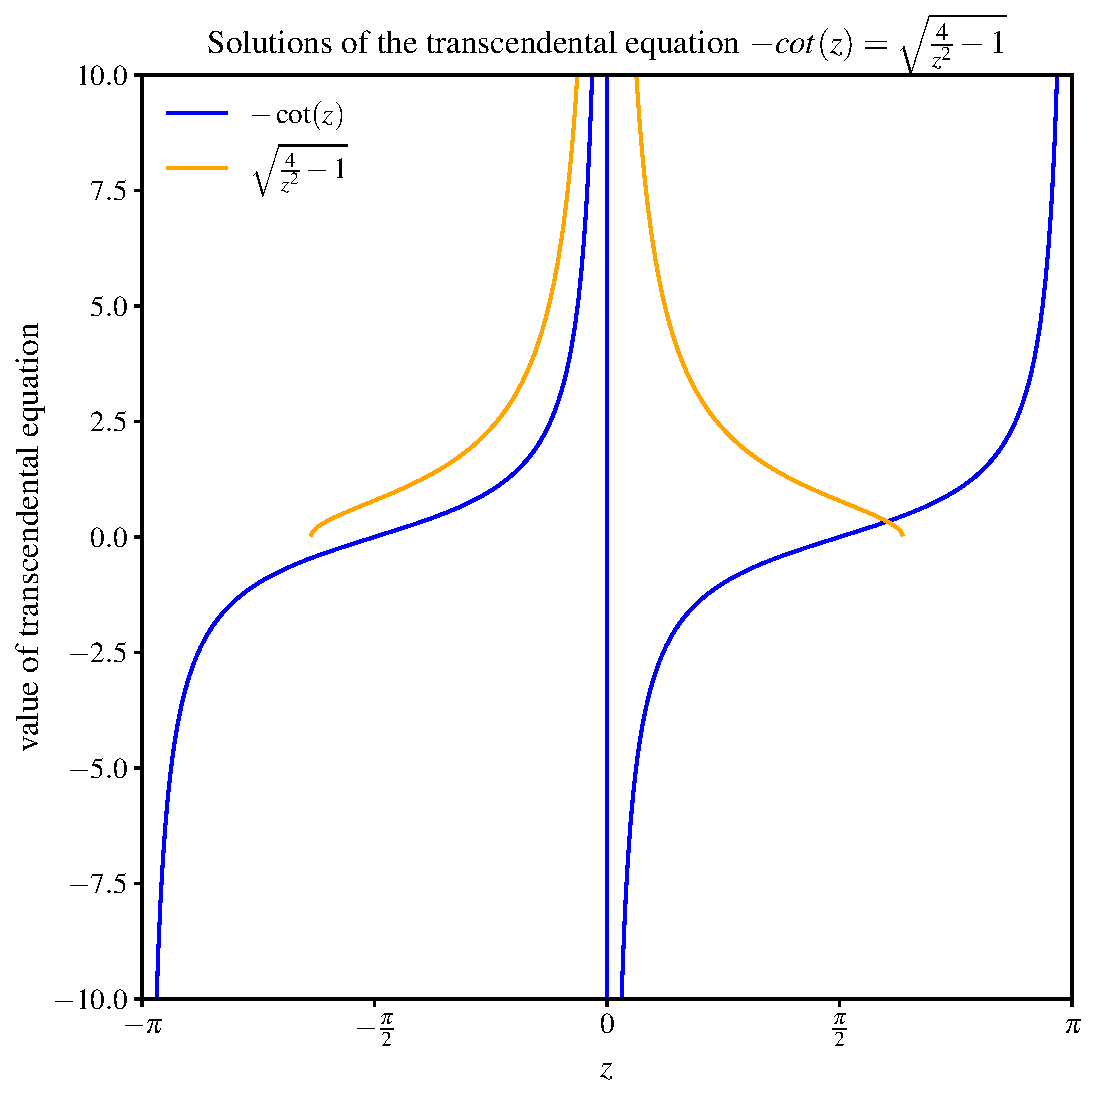
\includegraphics[width=0.7\textwidth]{figures/transcendental_equation.pdf}
    \caption{The left hand side (lhs) and right hand side (rhs) of the transcendental equation of the even wavefunctions.}
    \label{fig:tran}
\end{figure}
Shown in Figure \ref{fig:tran} is the intersections of the transcendental equation determining the number of bound states with odd wavefunctions for \(Z_0=2\). There exists one bound state wavefunction with an intersection approximately located at \(z=\pi/2\).

\vspace{\baselineskip}
\item Consider a particle interacting with the following potential energy landscape:
\[V(x) = \begin{cases}
\infty, & x < 0, \\ -V_0, & 0 < x < a, \\ 0, & x > a.
\end{cases}\]
\begin{enumerate}[label=(\alph*.)]
\item Determine the bound-state wavefunctions in three regions: (i.)~\(x < 0\), (ii.) \(0 < x < a\), and (iii.)~\(x > a\).
Note that this potential energy is not symmetric, so you cannot assume solutions will be alternatingly even and odd; instead, you must use the most general solution for the middle region's wavefunction.

This potential bears resemblance to the finite square well potential so we can use similar solutions for the wavefunction in region (ii.) and region (iii.). Furthermore, knowing \(\psi_\text{I}(x)=0\) because \(V_\text{I}(x)=\infty\) requires that the general solution of \(\psi_\text{II}(x)\) be equal to 0 at \(x=0\). This is only valid for the odd solutions found in problem 2 because it would require that \(D=0\) in Griffiths Equation 2.152. Thus,
\[\psi(x) = \begin{cases}
0, & x < 0, \\ C \sin(lx), & 0 \le x \le a, \\ F\exp(-\kappa x), & x > a.
\end{cases}\]

\item Apply appropriate boundary conditions at \(x=0\) and \(x=a\). Combine the results to determine the transcendental equation that governs the bound-state energies. Does it look familiar?

The boundary condition at \(x=a\), that \(\psi(x)\) and \(\diff{\psi}{x}\) are continuous, will result in the same transcendental equation as in problem 2! That is,
\[-\cot(z) = \sqrt{\frac{z_0^2}{z^2}-1}.\]

\end{enumerate}
\end{enumerate}
\end{document}
